\documentclass{article}
\usepackage[utf8]{inputenc}
\usepackage{graphicx}

\title{Oracle Application Exspress}
\author{Dinda Anik Masruro (1184003)}
\date{7 November 2019}

\begin{document}

\maketitle

\section{Membuat Aplikasi dengan APEX}
\subsection{Tuorial APEX}
\item https://apex.oracle.com/pls/apex/f?p=93074:LOGIN_DESKTOP:33096832912718:::::
\item 1. Pertama, buat dahulu workspace yang ingin di gunakan untuk membuat aplikasi pada APEX yaitu dengan cara kunjungi website https://apex.oracle.com/en/ lalu sign in.
\item 2. Lalu, isi semua data dengan benar, lalu login ke dalam workspace.
\begin{center}
    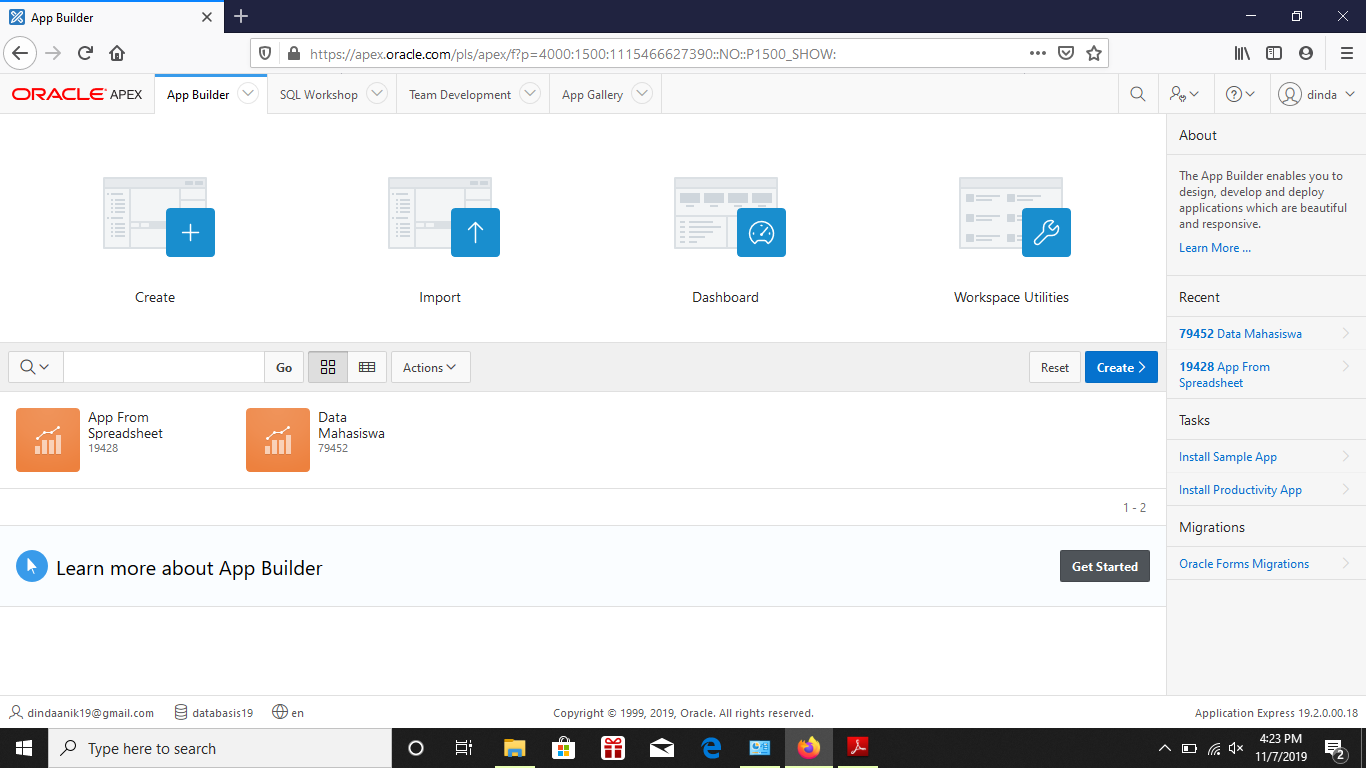
\includegraphics[width=10cm\textwidth]{gambar/1.png}
\end{center}
\newpage
\item 3. Setelah itu klik app builder dan klik create
\begin{center}
 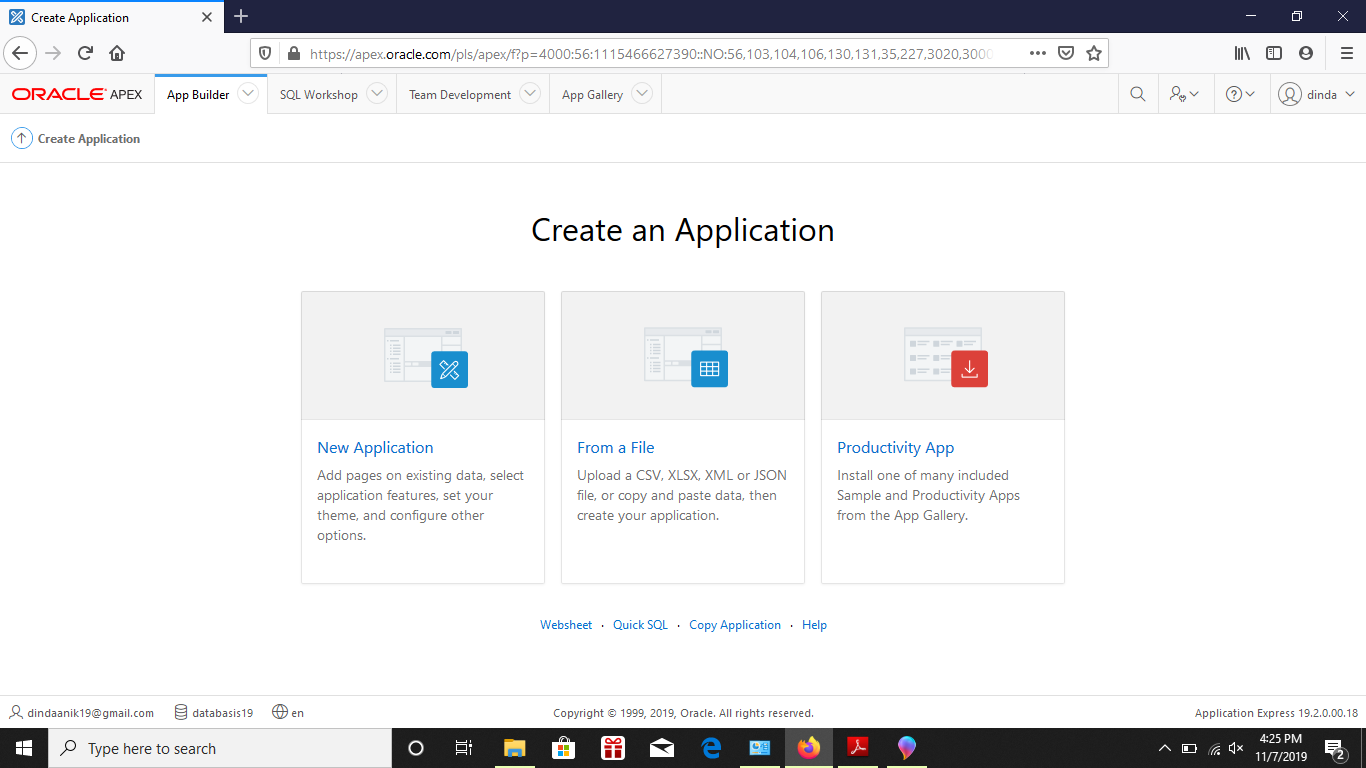
\includegraphics[width=10cm\textwidth]{gambar/2.png}
\end{center}
\item 4. Selanjutnya, klik From a File
\begin{center}
    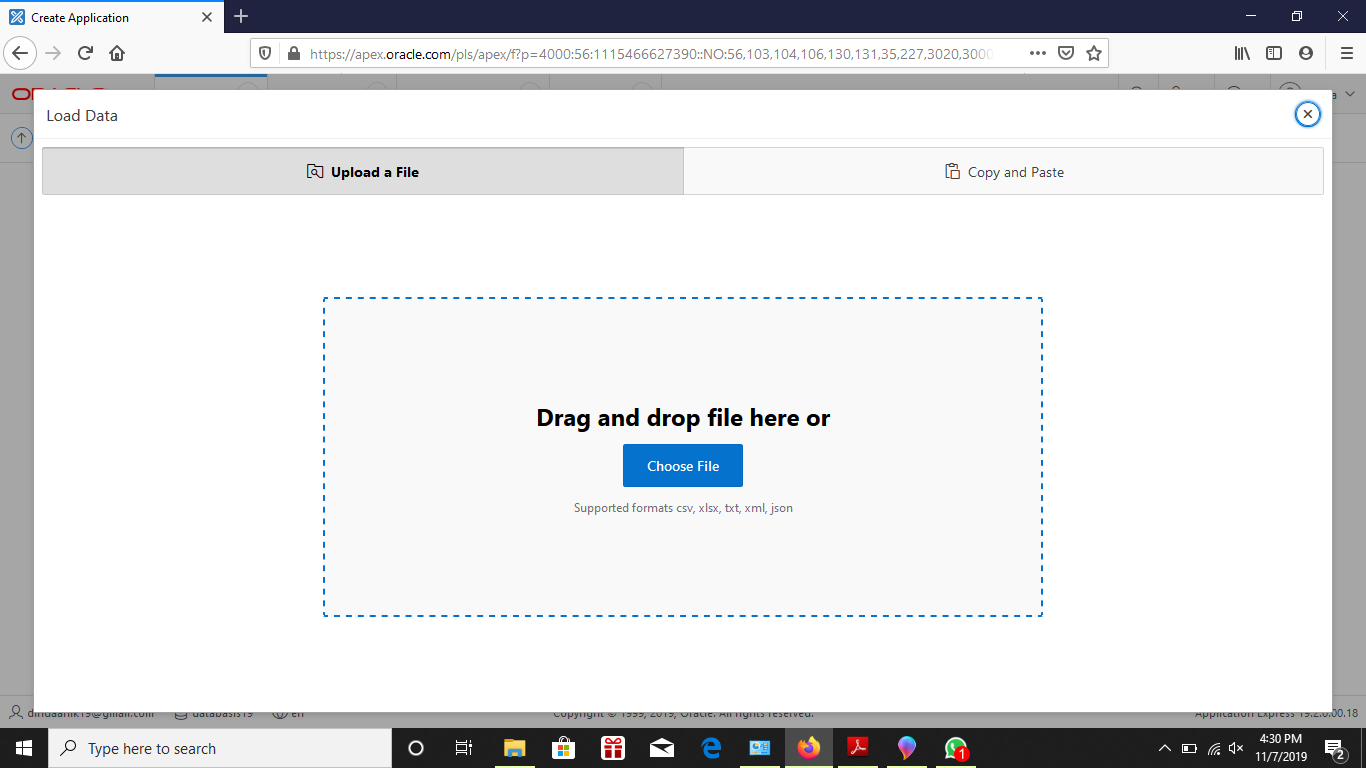
\includegraphics[width=10cm\textwidth]{gambar/3.png}
 \end{center}
 \newpage
 \item 5. Setelah kita pilih dan klik open.
\begin{center}
 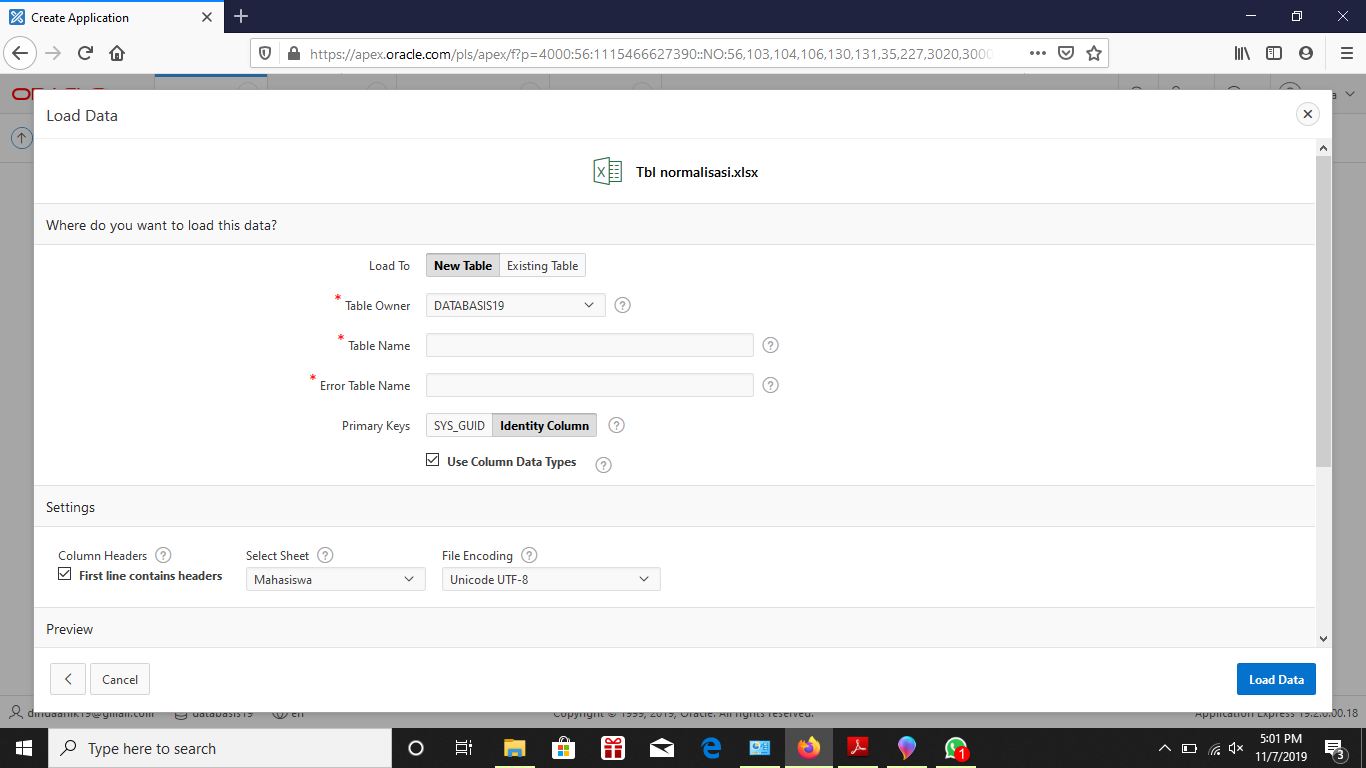
\includegraphics[width=10cm\textwidth]{gambar/5.png}
\end{center}
 \item 6. Setelah kita pilih selanjutnya kita masukkan nama tabelnya lalu klik fIeld error table name
\begin{center}
 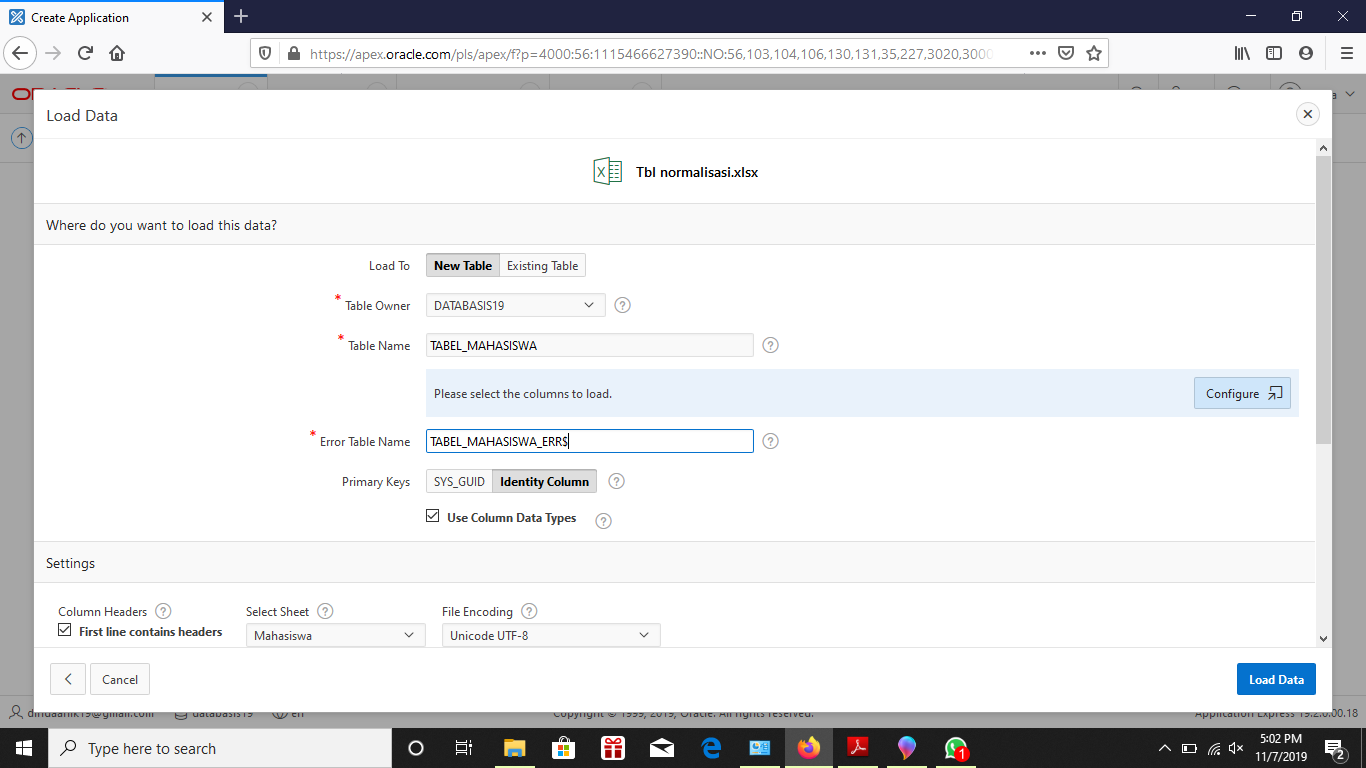
\includegraphics[width=10cm\textwidth]{gambar/6.png}
\end{center}
\newpage
\item 7. Klik confgure untuk memastikan bahwa atribut sudah benar
\begin{center}
 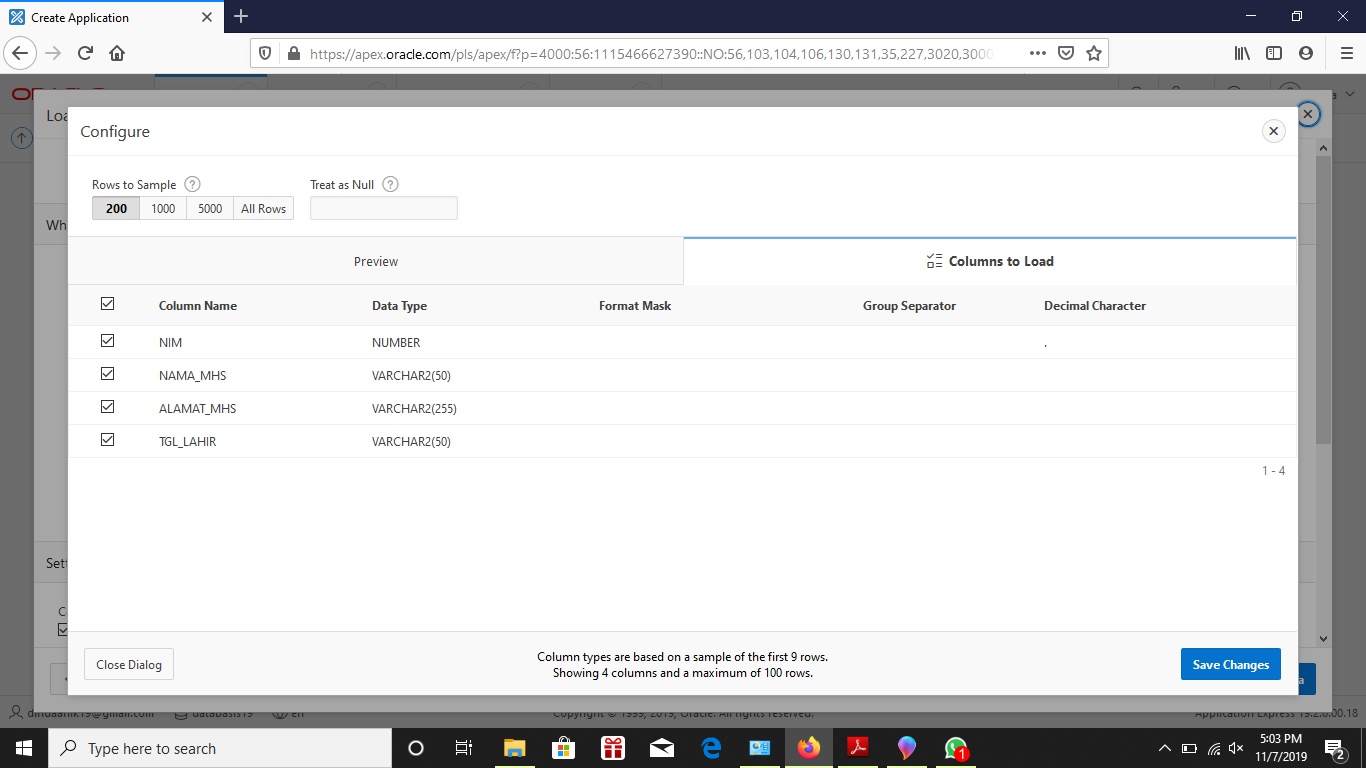
\includegraphics[width=10cm\textwidth]{gambar/7.png}
\end{center}
\item 8. Setelah itu klik save change. 
\begin{center}
 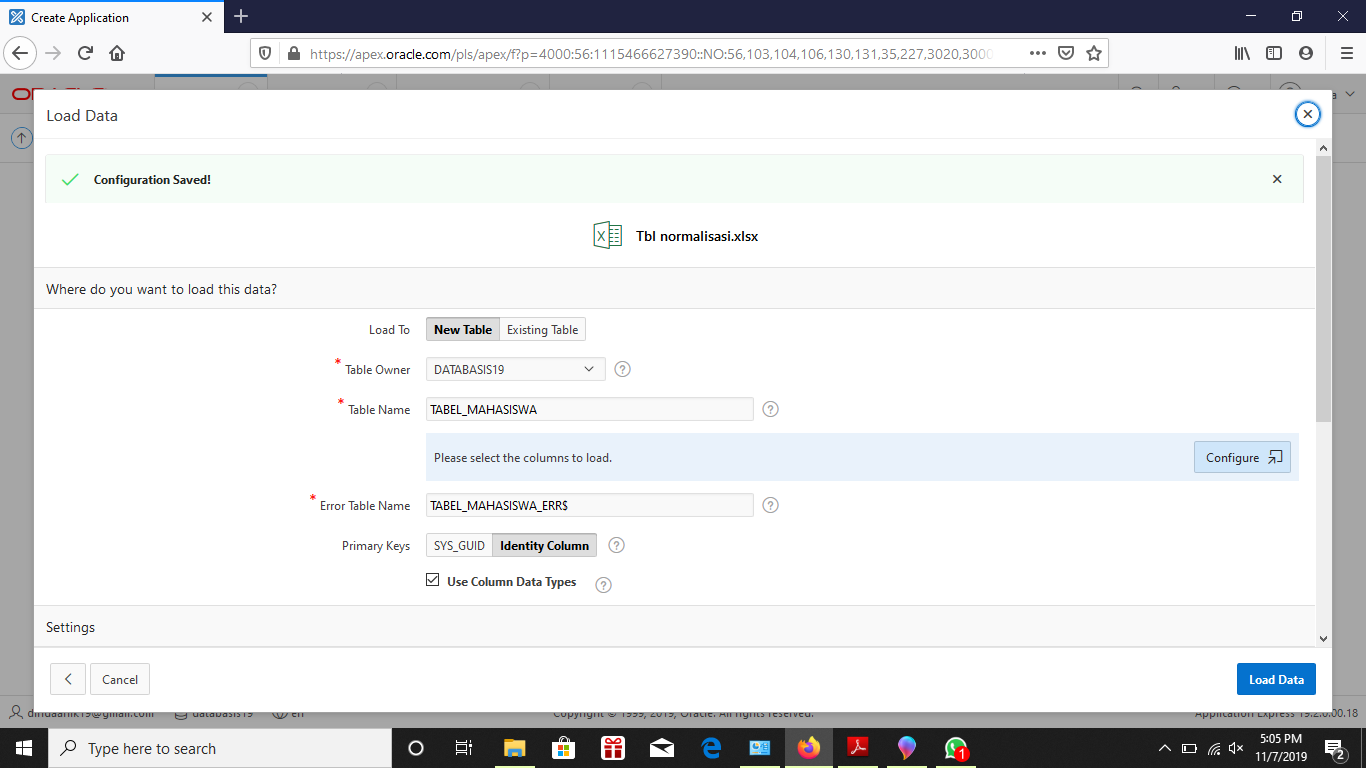
\includegraphics[width=10cm\textwidth]{gambar/8.png}
\end{center}
\item 9. Lalu klik load data dan tunggu hingga berhasil.
\begin{center}
 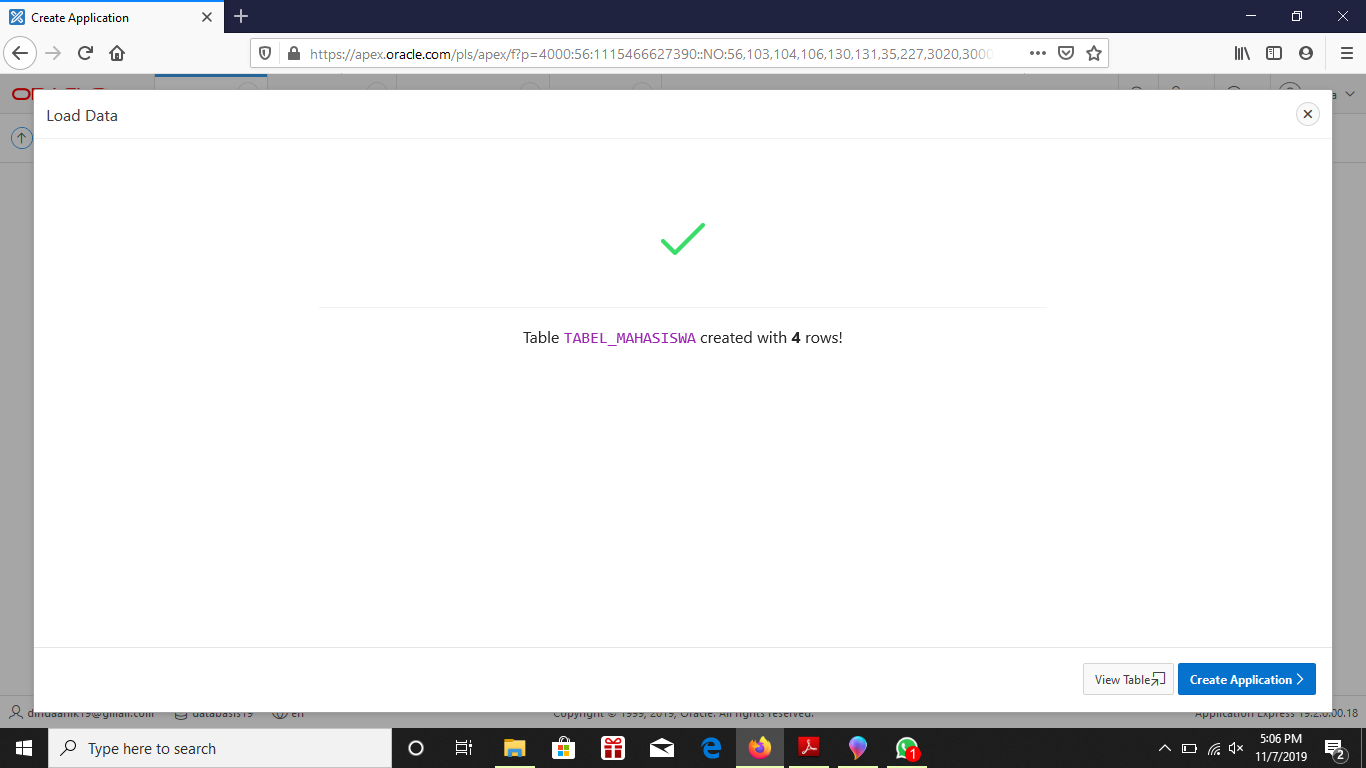
\includegraphics[width=10cm\textwidth]{gambar/9.png}
\end{center}
\item 10. Lakukan cara seperti di atas secara berulang dari tahap 3 hingga tahap 9 sesuai jumlah tabel yang diupload. Jika sudah akan melakukan penghapusan kolom ID, dan ini ID dapat otomatis oleh sistem apex jika di file tidak memiliki primary key. Setelah itu klik sql workshop lalu ke object browser
\begin{center}
 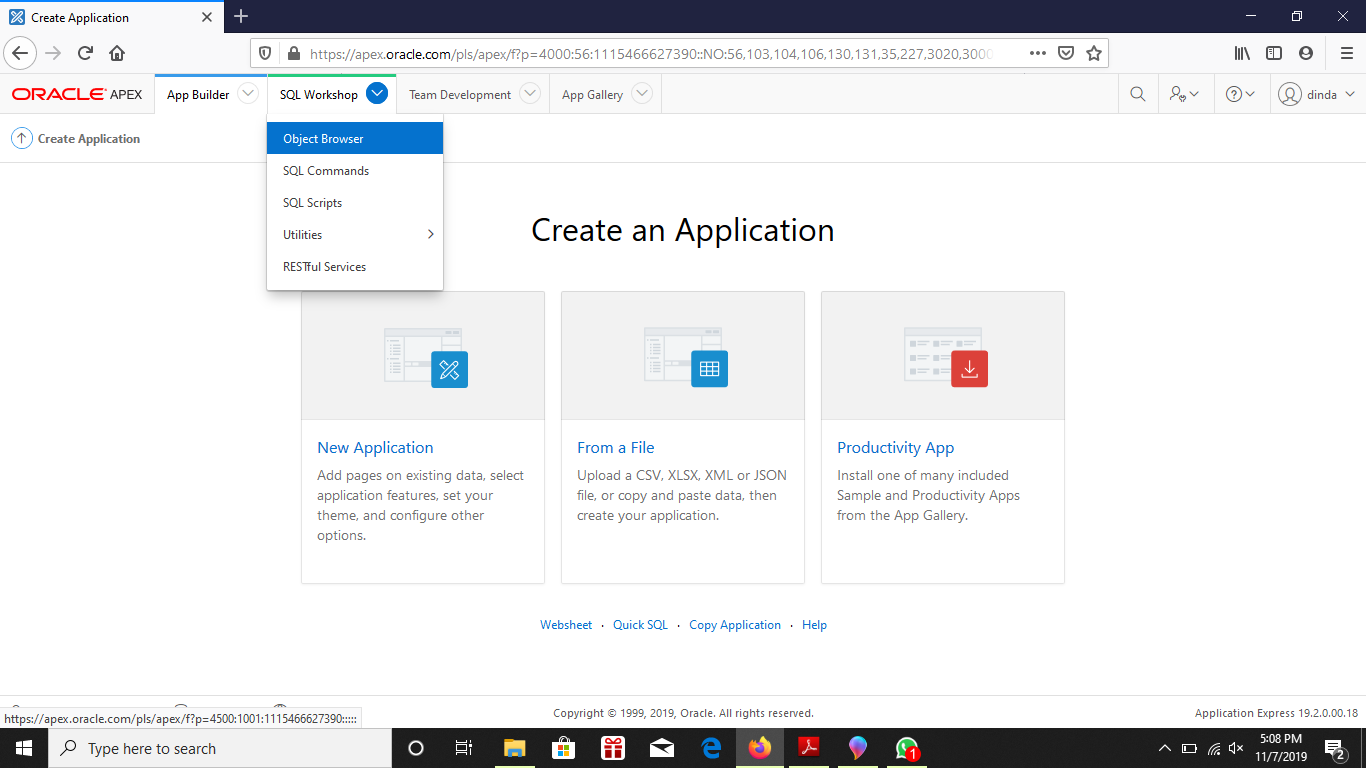
\includegraphics[width=10cm\textwidth]{gambar/10.png}
\end{center}
\item 11. Selanjutnya kita klik tabel yang ingin kita drop
\begin{center}
 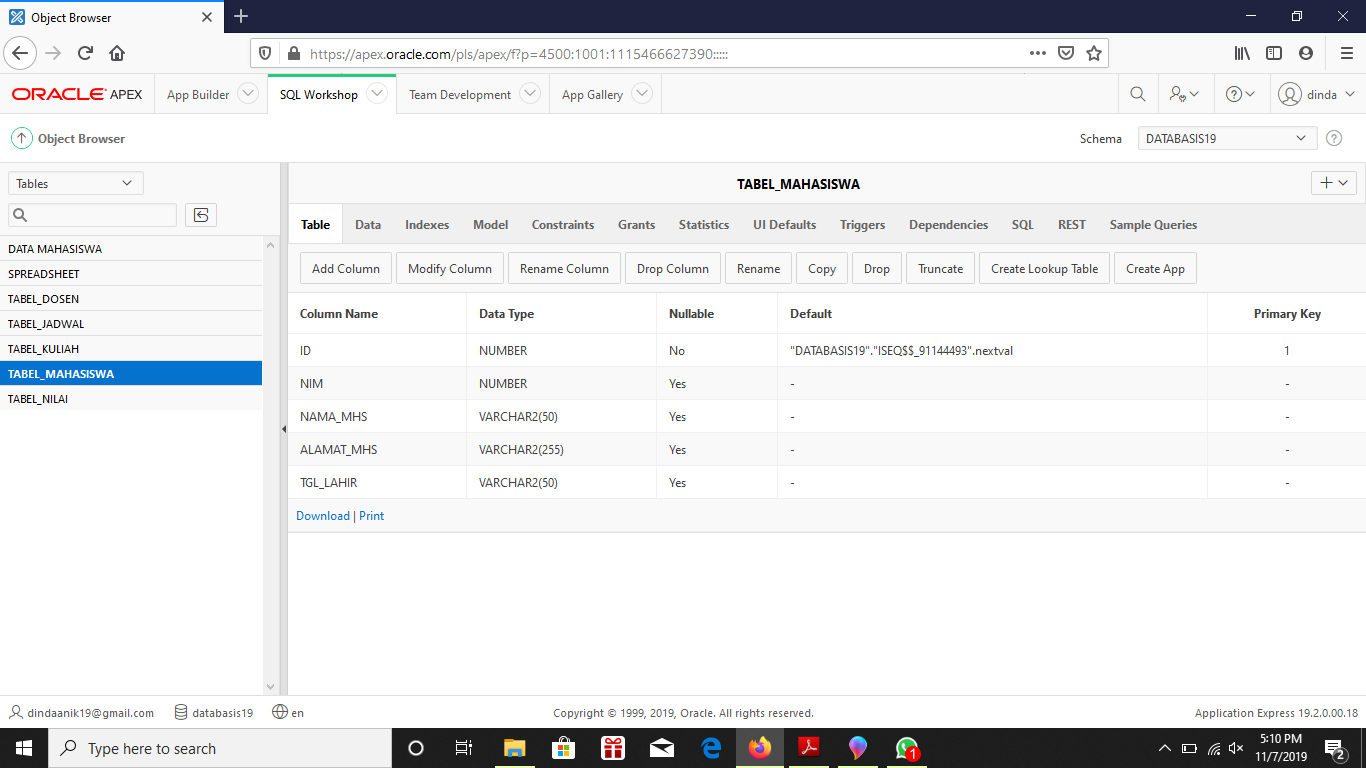
\includegraphics[width=10cm\textwidth]{gambar/11.png}
\end{center}
\newpage
\item 12. Kemudian klik Drop Column, lalu pilih kolom yang ingin di drop dan  klik drop lalu klik finish dan lakukan berulang hingga semua tabel terbebas dari primary key. Setelah itu akan add primary key setiap tabel yang telah diupload.
\begin{center}
 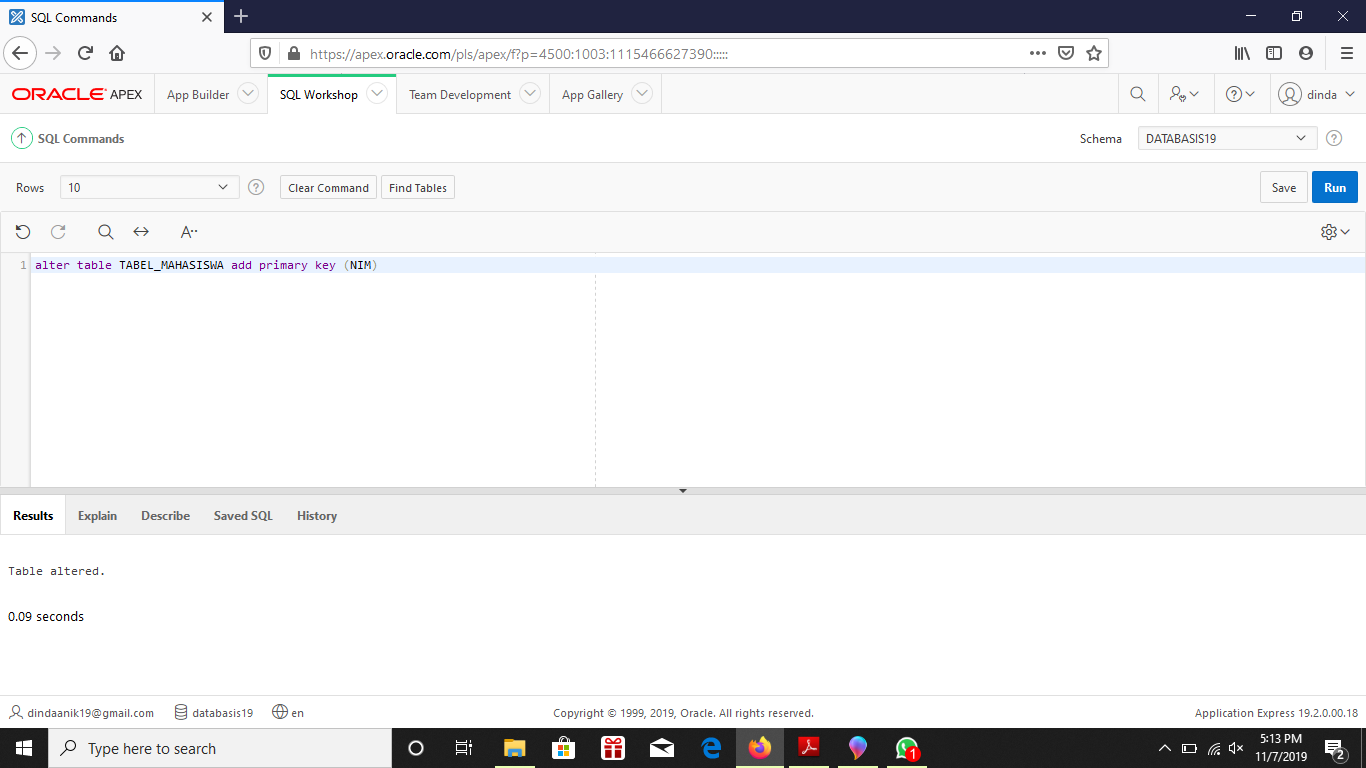
\includegraphics[width=10cm\textwidth]{gambar/12.png}
\end{center}
\item 13.Setelah itu kita run, tunggu hingga muncul pesan table altered. Langkah selanjutnya adalah cara merelasikan dua tabel, yaitu  mengketikkan query.
\item 14. Langkah selanjutnya ke app builder lalu klik create lalu klik new application
\begin{center}
    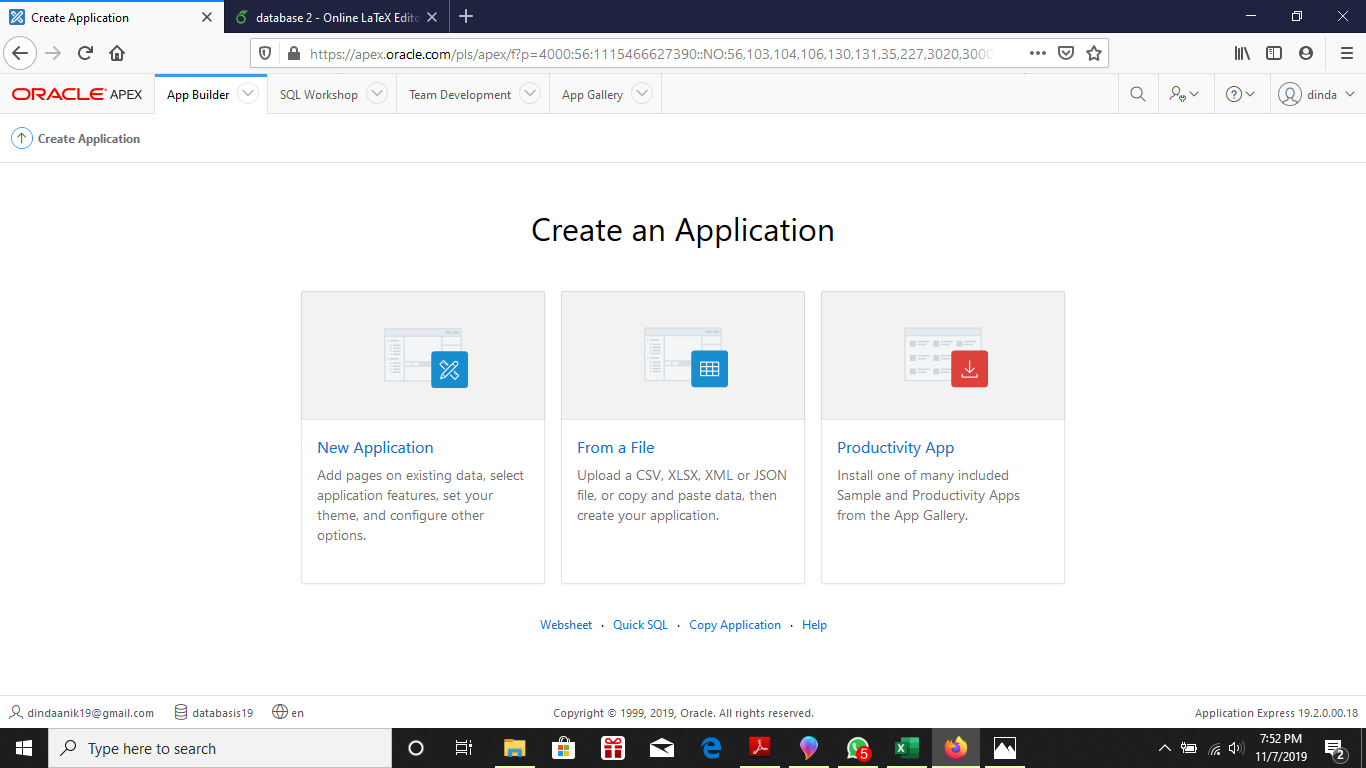
\includegraphics[width=10cm\textwidth]{gambar/15.png}
\end{center}
\item 15. Setelah itu add page
\begin{center}
 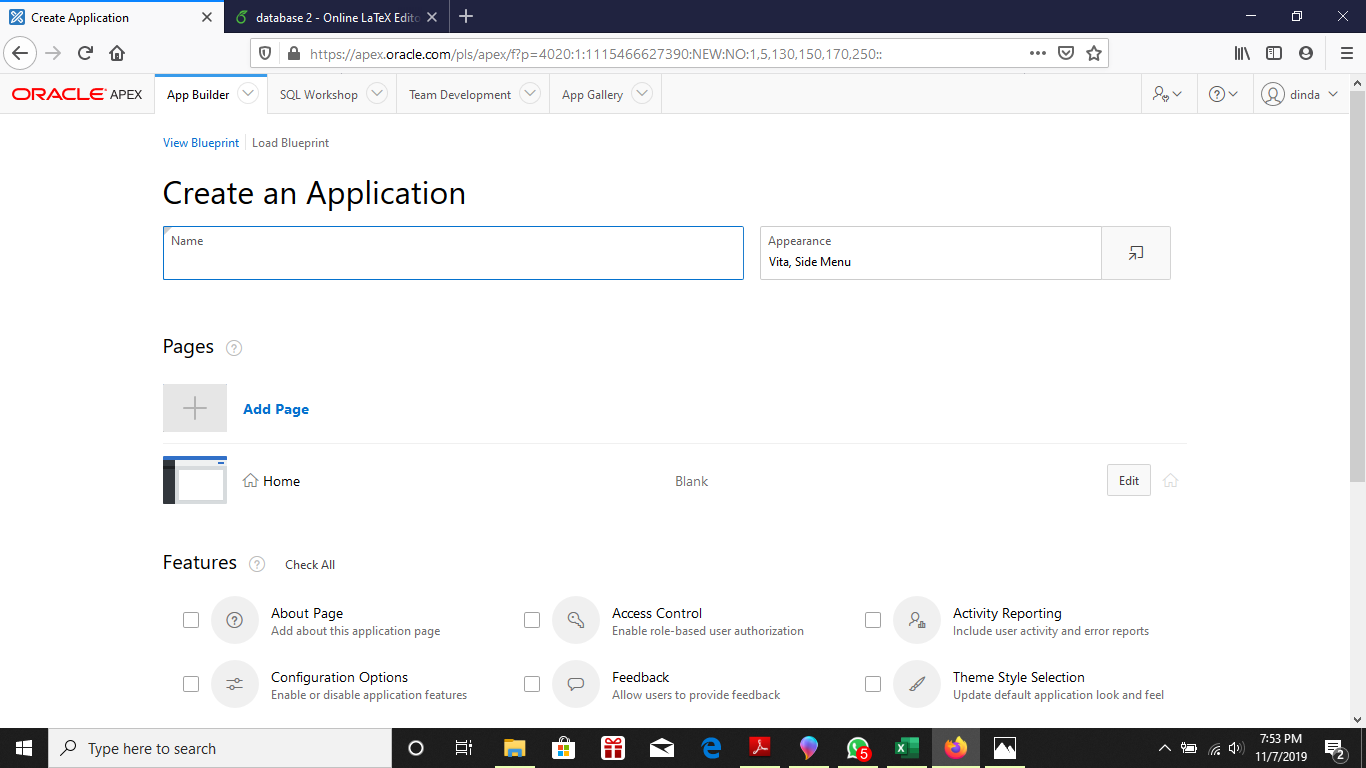
\includegraphics[width=10cm\textwidth]{gambar/16.png}
\end{center}
\item 16. Kita pilih form
\begin{center}
 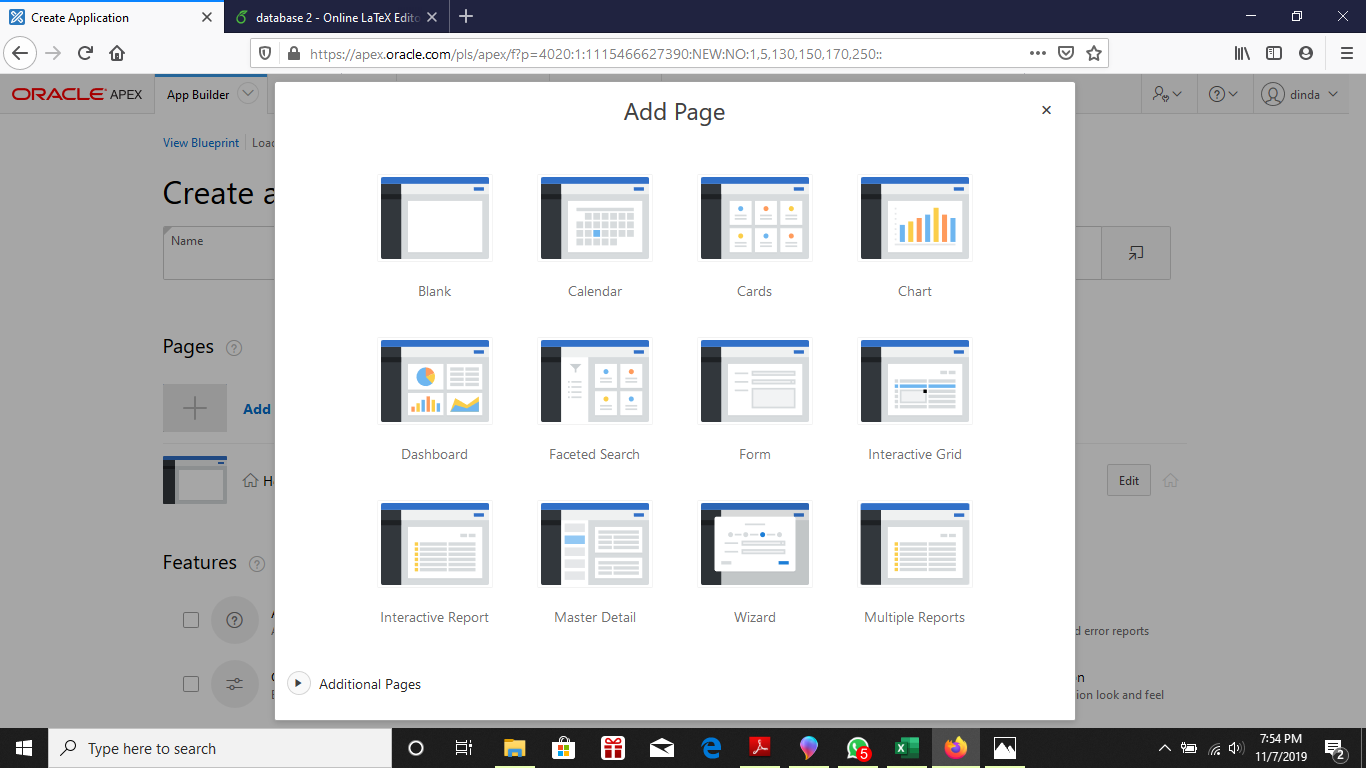
\includegraphics[width=10cm\textwidth]{gambar/17.png}
\end{center}
\item 17. Lalu klik select table, lalu pilih tabelnya
\begin{center}
 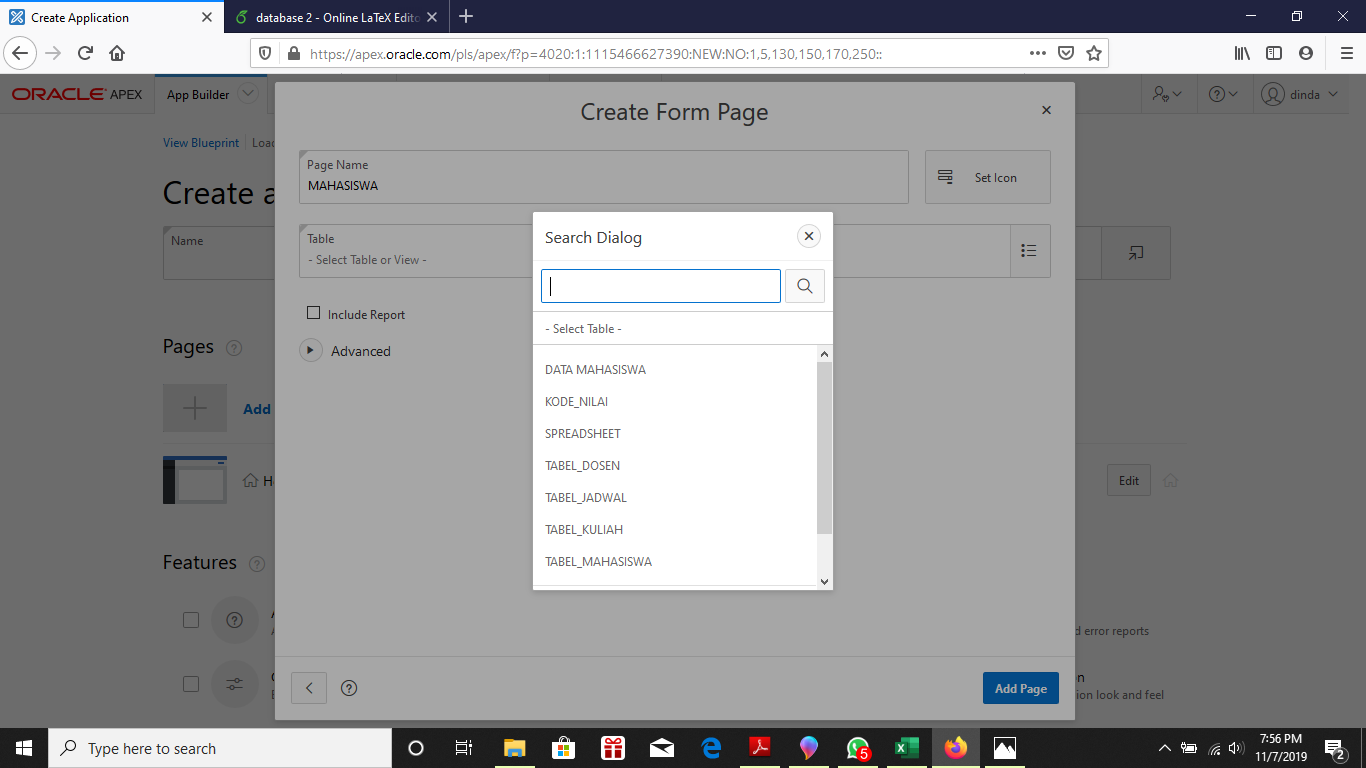
\includegraphics[width=10cm\textwidth]{gambar/18.png}
\end{center}
\item 18. Setelah itu kita isi page name lalu klik ok
\begin{center}
 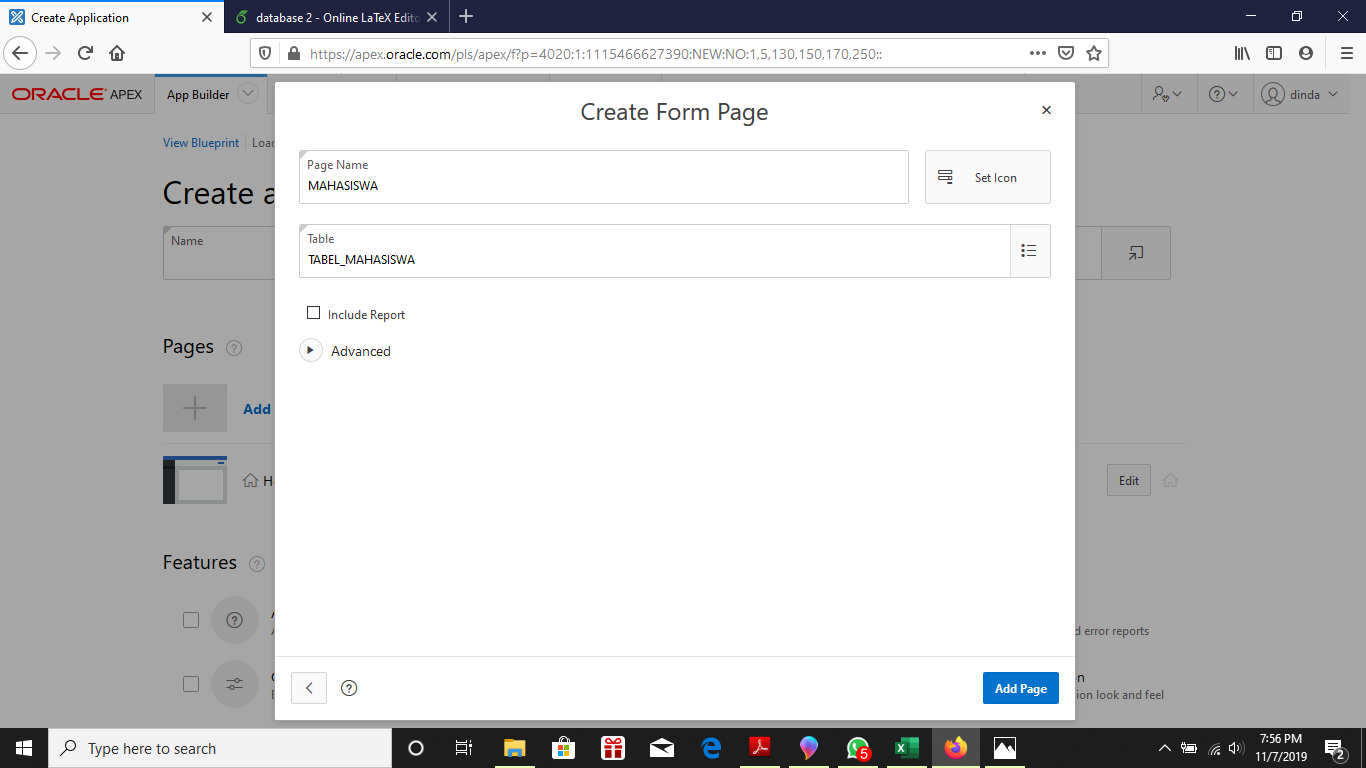
\includegraphics[width=10cm\textwidth]{gambar/19.png}
\end{center}
\item 19. setelah itu kita run application
\begin{center}
 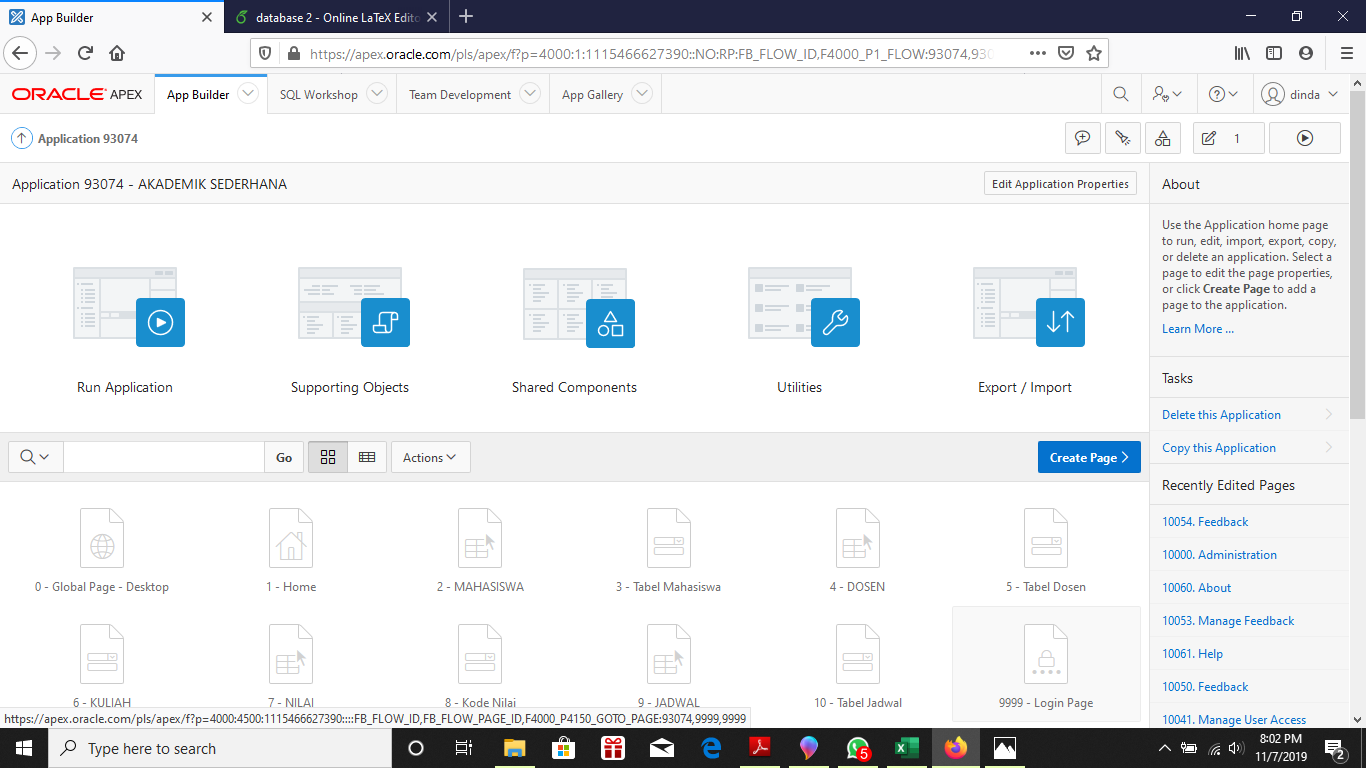
\includegraphics[width=10cm\textwidth]{gambar/20.png}
\end{center}
\item 20. Ini Merupakan User Interface
\begin{center}
 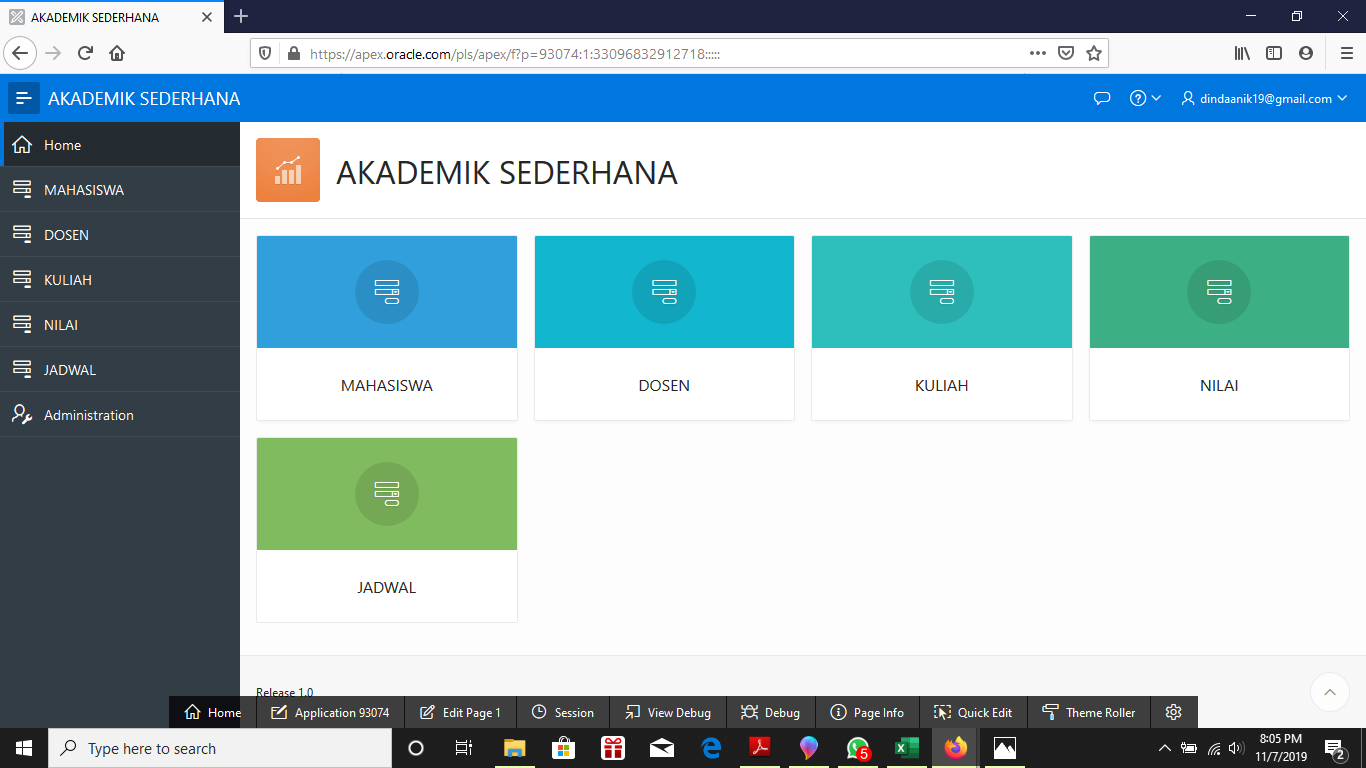
\includegraphics[width=10cm\textwidth]{gambar/21.png}
  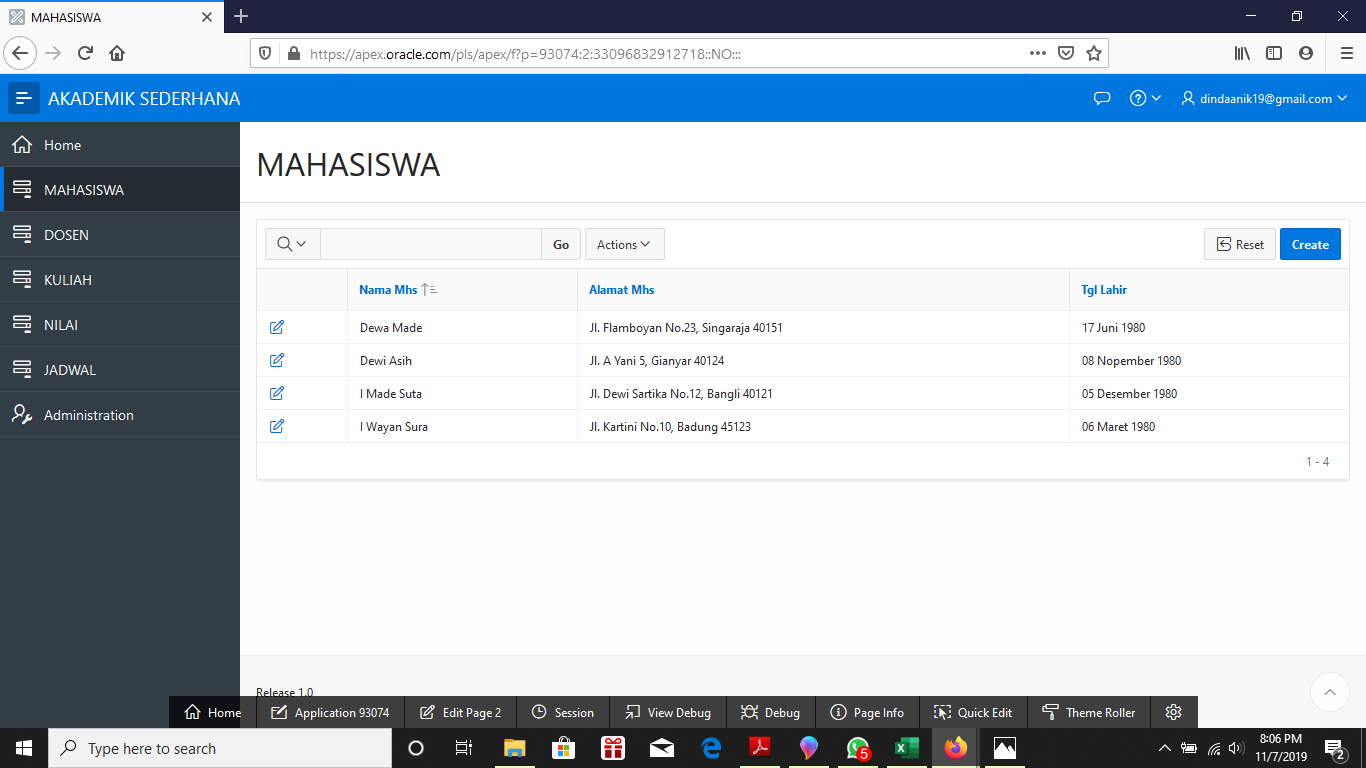
\includegraphics[width=10cm\textwidth]{gambar/23.png}
\end{center}
\item username: databasis19
\item password: dinda181205
\end{document}
